\subsection{团队架构}

    \subsubsection{队伍架构概述}
    
        \noindent
        \LTXtable{\textwidth}{table/3_managementStructure.tex}

        \noindent
        \LTXtable{\textwidth}{table/3_memberStructure.tex}

    \subsubsection{团队招募计划}

        \paragraph{招新渠道及招新方式分析}

            在招新渠道上,我们主要通过战队的公众号推文吸引新人,并请学院帮忙转发推文,同时私下请相关专业的同学转到专业班级群中。除此以外,我们也通过在线下招新摆摊发放传单、在校内张贴海报等途径进行招新。由于后两种是向校内同学无差别推送,不如招新推送有针对性。但线下摆摊气氛较为热烈,常常引人驻足围观,这也有利于 RoboMaster 赛事向不相关专业的群众宣传,提高其知名度。\par

            \subparagraph{机械组招新方式}

                招新流程分为多个阶段,确保选拔到具备全面素质和技能的优秀成员。具体流程如下:

                \setlist[itemize]{label=\raisebox{-1.2ex}{\scalebox{3}{$\textbullet$}}}

                \begin{itemize}
                    \item 首先,有意参加的新同学需提交报名表和个人简历,以展示个人基本信息和兴趣方向;
                    \item 其次,通过报名表和简历初步筛选后,我们将要求新同学自学相关方向,并提交学习计划、 学习内容以及链接的课程资源,例如在SW软件领域的学习教程、RoboMaster论坛链接,或其他关键领域的材料力学课程等。这一步主要考核新同学的自学能力和对所报名方向的热情。
                    \item 之后,选中的新同学将对论坛开源的机器人模型挑选感兴趣的模块,并完成一份分析报告,展示对模型的基本理解和认识。这有助于进一步评估新同学对机器人模型的逻辑思考和分析能力。
                    \item 然后,通过前述步骤的筛选,挑选出第一批同学后,进行SW软件的上机考试和有关于比赛规则及基本材料力学的笔试,以深入考核新同学对SW软件的熟练运用情况和对比赛的认识程度。通过提供零件工程图和装配图,限时三小时的上机和笔试考试,以评估新同学的建模能力和自学能力。 
                    \item 之后在第二轮中,筛选第一轮表现优异的同学,进行多对一的面试。这一轮的面试将聚焦于新同学的生理素质、心态品质,以及对比赛的热情和团队协作意识。 
                    \item 最终,根据整个招新流程的综合表现,确定入选机械组梯队的队员名单。这一过程将确保新队员在技术和团队合作方面都具备出色的素质,为团队的协同工作和未来比赛做好充分准备。
                \end{itemize}

            \subparagraph{电控组招新方式}

                电控组招新分多个阶段:

                \setlist[itemize]{label=\raisebox{-1.2ex}{\scalebox{3}{$\textbullet$}}}

                \begin{itemize}
                    \item 首先进行笔试,着重考察C语言基础和编程能力以及一部分的嵌入式知识,筛选第一批基础达标的人通过笔试。
                    \item 2.通过笔试的人会进行面试,面试会提问C语言、嵌入式的基础知识和对比赛的了解程度,但是着重考察对团队对开发对比赛的态度,通过面试的人员就成为悍匠战队的预备队员。
                    \item 3.预备队员会进入培训阶段。培训阶段会培训嵌入式基础和电控算法基础,然后根据培训进度发布阶段性任务;培训结束之后会对阶段性任务的完成度评分,会对评分不合格人进行筛选。
                    \item 通过培训的预备队员将会和其他组别的预备队员参与校内赛,校内赛进行期间将会对预备队员发布周期任务并对周期任务进行评分,筛选评分过低和态度不端正的人员。
                    \item 校内赛过后,留下的预备队员就会(以个人意愿优先)被分配到各个兵种进行后续学习,成为各兵种的预备开发人员,此时会发布新人的终期考核任务用于考察他们的实际开发能力。此后便协助各兵种的主力开发测试及维护,并且我们会筛选一部分出色的人员加入梯队,参与正式比赛。
                \end{itemize}

            \subparagraph{视觉组招新方式}

                \setlist[itemize]{label=\raisebox{-1.2ex}{\scalebox{3}{$\textbullet$}}}

                \begin{itemize}
                    \item 笔试:通过基础规则常识考核、c++考核等阶段性考核的方式逐层选拔,最终挑选一批能力优秀且有潜力的新人。
                    \item 最终会让新人写一个装甲板或者能量机关的识别程序,通过最终的考核即成为梯队队员。
                    \item 面试:面试着重考察临场反应能力和平时积累,通过面试的新人通常具有比较高的水准。
                \end{itemize}

            \subparagraph{硬件组招新方式}

                针对不同的技术需求,本赛季硬件组的招新考核部分与电控组分离。

                \setlist[itemize]{label=\raisebox{-1.2ex}{\scalebox{3}{$\textbullet$}}}

                \begin{itemize}
                    \item 参与者首先与电控组一同进行第一轮的编程题机考。
                    \item 而后经历为期半周的硬件通识考核.
                    \item 最后进行线下面试,三次考核分数经由不同权重组成最终得分.
                    \item 过者由主力队员组织培训后,成为梯队队员参与到日常维护与技术研发。
                \end{itemize}

            \subparagraph{运营组招新方式}

                随着深圳技术大学悍匠战队的不断发展与壮大,为了进一步提升战队运营效率,增强团队创新能力与竞争力,运营组在每学期初始都会开展新一轮招新活动。运营组招新旨在吸引一批具有创新思维、良好的沟通能力、扎实的专业技能及强烈责任感的大一新生加入悍匠战队,共同推动战队稳健前进。
                运营组主要从三个方向招收大一新生:

                \setlist[itemize]{label=\raisebox{-1.2ex}{\scalebox{3}{$\textbullet$}}}

                \begin{itemize}
                    \item 宣传部:负责线上线下活动的策划与微信公众号等平台的内容策划、编辑与发布,提高悍匠战队活跃度。
                    \item 财务部:对战队资金流动等运营数据进行监控、分析,为战队决策提供数据支持。
                    \item 设计部:负责周边产品的设计。
                    \item 在明确招新目标、时间安排等后,运营组利用海报、宣传视频等,通过学校官网、微信公众号、QQ群等社交平台发布招新信息,扩大影响力。同时运营组成员会在食堂、图书馆、教学楼等人流密集区域张贴招新海报,设置咨询摊位,面对面解答疑问。
                    \item 新生投递报名资料后,运营组将对申请者的基本信息、专业技能、过往经历等进行初步筛选,同时布置考核作业与提交期限。在收到申请者考核作业后,运营组将通过微信群通知入选者参加面试,明确面试时间、地点及注意事项。
                \end{itemize}

    \subsubsection{团队培训计划}

        \paragraph{机械组}

            \subparagraph{培训形式}

                机械组对新人的培训主要采取一对一导师制,按新人意愿优先原则分配新人到各个项目组中,在设计时进行讲解,也会不定时分配小任务给新人完成,让新人参与到整个项目中;不定期开展机械组内会议,也是作为机械组新人培训会,激发新人的自主学习能力,师傅领进门,修行在个人,新人们会到论坛上爬取开源,或者主动询问老队员,最后将调研后的知识写成感悟提交给负责人检查,这样做提升了新人寻找资料来完成任务的能力;举行新人校内赛,让各车组新人初次体验如何通过团队合作、相互沟通完成车辆的设计的装配,进一步激发新人对比赛的热情,同时也提高他们的软件熟练度和设计思维及装配能力。
  
            \subparagraph{培训安排}

                \LTXtable{\textwidth}{Group/3.7.1.2_mechanicalTraining_arrangement.tex}

        \paragraph{电控组}

            \subparagraph{培训形式}

                \setlist[itemize]{label=\raisebox{-1.2ex}{\scalebox{3}{$\textbullet$}}}

                \begin{itemize}
                    \item 电控组对新人的培训方式主要采取导师制,授课加任务验收的方式。
                    \item 在这个培训体系中,一个导师将会辅导一组(3到4名)新人,负责引导他们解决在学习过程中遇到的困难和疑惑,导师一般由老队员担任,旨在通过他们丰富的经验和知识帮助新人更快的入门;
                    \item 导师还担任着监督者的任务,监督新人及时参与培训并按时完成任务,并观察他们的态度。
                    \item 此外,定期授课的方式将比赛中所运用的各项技术拆分细化后融合进若干课程中,经过课程讲解基础知识,再布置验收任务,任务难度由易至难呈阶梯式上升。
                    \item 除了定期授课,定期布置任务并进行任务验收是必不可少的一环。导师会对新人完成的任务进行评估,提供具体的反馈,并根 据需要调整培训计划。这种及时的反馈机制有助于新人快速纠正错误,不断改进自己的表现。当所有培训课程结束后,会筛选一部分态度不端正和培训任务完成度过低的新人。
                    \item 之后新人将会参与校内赛体验真实的开发和备赛过程,校内赛期间会周期性布置校内赛的任务并对任务评分以及对新人的态度做评估,筛选不过关的人员。
                    \item 校内赛过后新人(以个人意愿优先)将会被分配到各个兵种进行后续学习,此时将会发布终期考核任务考察他们的实际开发能力。
                    \item 此后便协助各兵种的主力开发测试及维护机器人,逐渐熟悉开发流程和积累调试和开发经验,最终达到可以独自承担机器人控制部分的所有任务的目标。
                \end{itemize}

            \subparagraph{培训安排}

                \LTXtable{\textwidth}{Group/3.7.2.2_electricalTraining_arrangement.tex}

        \paragraph{视觉组}

            \subparagraph{培训形式}

                视觉组技术培训旨在提升学员在 C++、OpenCV 和 Linux 环境下的开发能力,通过多方位的培训形式,使学员能够在实际项目中熟练运用所学知识。将以授课、考核、作业、项目的形式进行培训。\par
                在第一轮选拔中,我们将进行 C++考核,通过对新生的笔试和面试评估,选取表现突出的新生作为预备队员。这些预备队员将进入下一轮的培训阶段,由主力队员亲自进行指导和培训。\par
                在培训过程中,我们将设定多个阶段性考核,以评估预备队员的学习进度和技能掌握情况。及时发现培训中出现的问题、提供针对性的帮助,并确保每位预备队员都能够逐步成长和适应团队的需求。 \par
                经过全面的培训和阶段性考核后,预备队员将参与到最终考核中。通过这一环节的评估,我们将选定表现出色的成员,正式纳入梯队,成为视觉开发团队的一员。\par
                
                \setlist[itemize]{label=\raisebox{-1.2ex}{\scalebox{3}{$\textbullet$}}}

                \begin{itemize}
                    \item 授课:每周定期授课,介绍新知识点和技术。提供示例代码和案例,帮助学员理解和应用所学内容。
                    \item 答疑:新人可以线下来实验室学习并互相交流或者找主力队员答疑。
                    \item 考核:定期小测验,检查学员对于每个知识点的理解程度。中期项目考核,要求学员完成一个小型项目,运用所学技能。
                    \item 作业:每节课后布置相应的作业,巩固学员的学习。作业涵盖编程练习、问题解决和小项目任务。
                    \item 实际项目:通过实际项目锻炼学员的实际开发能力。项目中模拟团队协作和开发流程,培养团队协同能力。
                \end{itemize}

            \subparagraph{培训安排}

                \LTXtable{\textwidth}{Group/3.7.3.2_visualTraining_arrangement.tex}

        \paragraph{硬件组}

            \subparagraph{培训形式}

                硬件组对新人的培训方式主要采取阶段性任务考核,分层渐进式完成指定目标。吸取上赛季培训周期过长的问题,本赛季在招新阶段融入了通识考核,新人业已完成基础知识的扫盲。同时,我们新开展第一届校内赛。校内赛旨在培养新成员的团队合作精神,面对技术挑战时的问题解决能力。在校内赛中,明确团队分工,让每个成员都能发挥作用。老成员负责定期验收本阶段任务,并进行评估,提供具体的反馈。由此新成员能够在短期经历完整的备赛体验,对悍匠团队和Robomaster赛事的认知亦更上一层。

            \subparagraph{培训安排}

                \LTXtable{\textwidth}{Group/3.7.4.2_hardwareTraining_arrangement.tex}

        \paragraph{运营组}

            \subparagraph{培训形式}

                运营组培训形式为各部门负责人牵头,向新成员讲解工作内容与运用到的相关软件,并每周进行相应课时的技能培训,在为期一月的培训结束后对新成员开展考核。在考核开始前,培训负责人应清晰地向新生解释考核的内容、评分标准以及注意事项。培训负责人应保持耐心,给予他们充分的展示机会,并在必要时提供适当的指导和鼓励。培训负责人要及时给予新生反馈,既包括他们表现优异的地方,也包括需要改进的地方。对于不足之处,尽量提出具体的、建设性的建议,帮助他们明确改进的方向和方法。在考核结果之外,培训负责人应更关注整个考核过程中新生的学习和成长,鼓励他们从每次尝试中汲取经验,不断完善自己,而不是仅仅追求最终的考核成绩。

            \subparagraph{培训安排}

                %\LTXtable{\textwidth}{Group/3.7.5.2_operatorTraining_arragement.tex}

                \setlist[itemize]{label=\raisebox{-1.2ex}{\scalebox{3}{$\textbullet$}}}

                \begin{itemize}
                    \item 鉴于大学生普遍缺乏财务实践经验,运营组财务部将展开“一对一”示范,以老队员带动新队员的形式,开展财务基础知识教学,采用案例分析、模拟演练等方式,使新成员能够初步掌握财务管理的基本技能。
                    \item 同时,针对设计岗位的新成员,策划部将开设Adobe系列设计软件(如Photoshop)教学,通过线上教程、实操练习及小项目设计,快速提升其设计技能。
                    \item 除此之外,为了积累宣传部成员的实战经验,将由宣传部新成员组织运营组内部的小型项目,如校园宣传活动、团队建设等,让成员在实战中积累经验,提升项目管理、团队协作及问题解决能力。
                \end{itemize}

    \subsubsection{团队架构梳理}

        \begin{figure}[H]
                    \centering
                    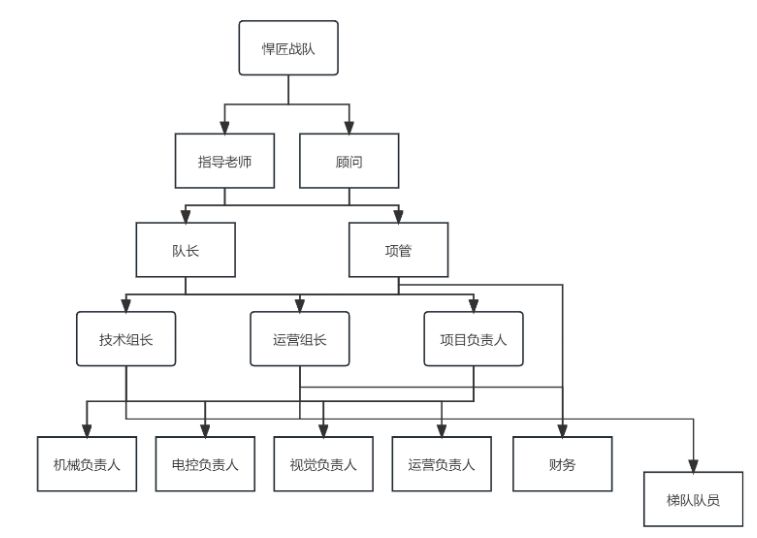
\includegraphics[height=0.9\textwidth]{figure/teamStructure_review.png}
                    \hspace{0.5em}
                    \caption{\textbf{\zihao{-4}\textbf{组织架构示意图}}}
                    \label{fig:teamStructure_review}
        \end{figure}